\subsection{Project Lifecycle and relevance}

This project is the first iteration of the university building a downwind vehicle. The current project aims to design and manufacture a vehicle that can be tested in at University facilities. There is no previous work on this vehicle in the university and within academia there are still debates as to whether the vehicle is physically possible and what fundamental concepts are at work with the vehicle in motion. A spotlight has been given to this type of vehicle recently due to the Veritasium YouTube video but many academics have rejected the abilities of blackbird to go faster than the wind. We aim to understand the workings of a downwind faster than the wind vehicle and begin an iterative method for projects within the university looking at downwind faster than the wind motion.

\subsection{Project Context}

With the global transportation market moving towards more sustainable forms of travel, all methods for generating thrust to power the future of motion have to be considered. The potentially self-sustaining nature of these vehicles offer significant opportunities for transportation companies to solve the environmental issues that are currently being faced by the planet. The vehicles in discussion are still early in development but a significant input into design could see many aspects of these vehicles implemented into sustainable travel in the future. The mechanical systems involved with these vehicles are not only limited too land vehicles, with boats being able to use these systems for propulsion when travelling. The abilities of these vehicles are promising and could offer significant solutions to the global problem of climate change. The project aims to analyse and discover the potential issues with designing this type of vehicle and give feedback on the limitations of building a vehicle such as this.

\subsection{Project Stakeholders}

See Table \ref{}.

\onecolumn
\newcommand\x{3.5cm} %set cell width
\begin{table}[p]
    \centering
    \begin{tabular}{|m{5cm}|m{\x}|m{\x}|m{\x}|m{\x}|m{\x}|m{\x}|m{\x}|m{\x}|}
      \hline
      \textbf{Design} &
      \textbf{Cost} &
      \textbf{Aesthetics} &
      \textbf{Modularity} &
      \textbf{Manufacturability} &
      \textbf{Safety} &
      \textbf{Performance} &
      \textbf{Complexity} &
      \textbf{Durability} 
      \\ \hline
      
      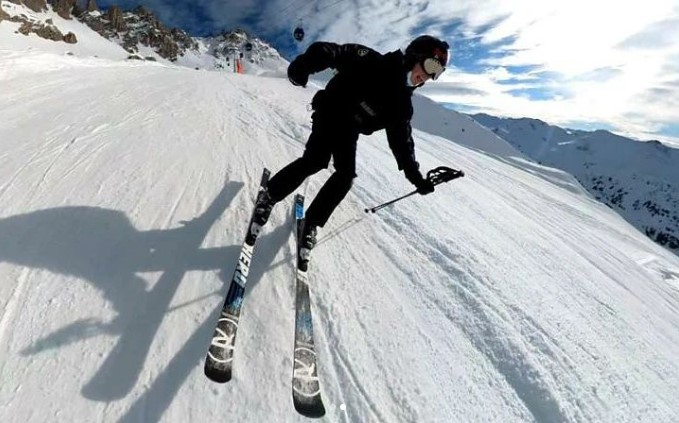
\includegraphics[width=\linewidth]{images/placeholder.jpg}
      &
      The cost of this vehicle could be larger than the other vehicles due to the aerodynamic body of the vehicle and the fact that there are two propellers. The dual prop design would also increase the amount of components in the drivetrain, increasing the cost.
      & 
      The finish is relatively clean for this vehicle, which improves the overall aesthetics. From analysis the streamlined body of the vehicle would add significant designing, to the project. 
      &  
      The drivetrain of this vehicle looks relatively modular, with the main structure being connected with bolts. The two-propeller system reduces the modularity of the vehicle.
      & 
      The two propellers would be able to be manufactured in tandem, but a significant amount of manufacturing would have to be completed to finish the vehicle.  
      &  
      The vehicle looks relatively stable, although the propeller looks relatively large in comparison to the vehicle which could cause oscillatory issues.
      &  
      The two-propeller system would generate a significant amount of thrust. 
      &  
      The vehicle is very complex with two propellers adding significant design for the drivetrain and the aerodynamics of the vehicle. 
      &  
      The vehicle has a lot of aerodynamic components that could be broken easily and would need to be replaced. Initially designing the vehicle for durability will therefore help improve the project, especially with us focussing on durability.
      \\ \hline
      
      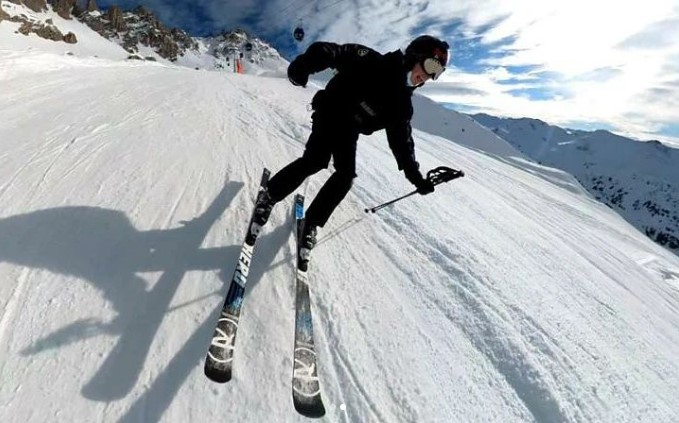
\includegraphics[width=\linewidth]{images/placeholder.jpg}
      &
      This vehicle looks very expensive due to the slick and streamlined nature of the body. The wheels are solid on this vehicle which would increase the expense of the vehicle significantly.
      &  
      The vehicle looks very aesthetically pleasing with the enclosed cockpit for the driver. The wheel covers add more to the design and make the vehicle look well engineered. 
      &  
      This vehicle doesn't look very complex. This is probably due to the fact that this vehicle is near the end of the design process and all components have been tested multiple times. 
      &  
      This vehicle will be difficult to manufacture. The aerodynamic body will have been made from a composite and the translucent window at the front will have been difficult to create. 
      &  
      This vehicle looks safe due to its enclosed cockpit design. The vehicle looks stable and there are obvious safety concerns that have been addressed on the vehicle. 
      &  
      This vehicle looks like it would performance well aerodynamically. The solid wheels will reduce the unpredictable nature of the wheels but will require additional suspension for the vehicle to run smoothly on the road. 
      &  
      The drivetrain system for this device looks like a shaft drive due to the thin pole supporting the vehicle. 
      & 
      As with the other vehicles, the outer casing will cause significant issues with durability, especially as composites can break with impacts. The wheels on this vehicle are an interesting prospect. 
      \\ \hline
      
      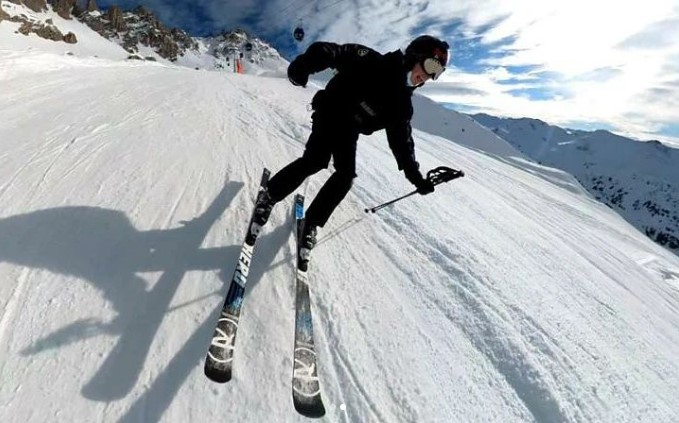
\includegraphics[width=\linewidth]{images/placeholder.jpg}
      &  
      This is the main vehicle that started the downwind faster than the wind theory. The propeller on this vehicle is large, therefore will cost a lot, adding to the already complex body.
      &  
      This vehicle looks relatively bulky but the significant aerodynamic components help improve the aerodynamics significantly. 
      &  
      As the vehicle has significant aerodynamic components that have been improved over a large amount of time, meaning most of the parts aren't replaceable. This vehicle isn't modular, and therefore takes a lot of work to maintain.
      &  
      Due to the complex components on this vehicle, this vehicle will be difficult to manufacture. On the whole the vehicle is complex to manufacture and is not a good vehicle to base our vehicle on.
      &  
      The YouTube video on this vehicle show significant oscillation when the propeller is moving quickly. The vehicle is not completely safe and has systems involved to stop the vehicle. Our vehicle is unmanned; therefore, these concerns will not be as significant. 
      &  
      This vehicle has shown incredible performance with good ability going upwind and downwind. The chain system on the vehicle provides significant tension for the propeller and spins and provides thrust at most speeds. 
      &  
      The vehicle is very complex in both aerodynamics and functionality. The vehicle can fold in half due to its size and need to be transported. The drivetrain of the vehicle although hidden is very complex and has been worked on for a long time.
      &  
      The vehicle is very large and components are state of the art for the vehicles, suggesting that they are not easily replaces. The vehicle frame is mechanical and therefore is prove to failure, and the structure is built from wood which with an impact could break 
      \\ \hline
    \end{tabular}
    \caption{Previous attempts at downwind-faster-than-the-wind vehicles}
    \label{tab:prevAttempts}
\end{table}
\twocolumn % From 1.introduction.tex

\onecolumn
\begin{table}[p]
\caption{Project stakeholders}
\label{tab:stakeholders}
\centering
\begin{tabular}{|
>{\columncolor[HTML]{\CellColor}}l |p{13cm}|p{13cm}|}
\hline
\cellcolor[HTML]{\CellColor} &
  \cellcolor[HTML]{\CellColor}\textbf{Specific   Information Needs} &
  \cellcolor[HTML]{\CellColor}\textbf{Stakeholder   needs and Interests} \\ \cline{2-3} 
\multirow{-2}{*}{\cellcolor[HTML]{\CellColor}\textbf{Project stakeholder name}} &
  \cellcolor[HTML]{\CellColor}\textbf{Types \& Frequency of   Communication} &
  \cellcolor[HTML]{\CellColor}\textbf{Specific areas of interest and participation} \\ \hline
\textbf{Supervisors} &
  Organising weekly meetings with the project supervisors and giving them presentations on the progress of the project in each period was key to the progress of the project. Asking questions and receiving feedback on progress allows for the supervisors to provide detailed analysis and suggestions for improvements for the project. The supervisor's interest in the project is derived from their involvement in the Engineering discipline as researchers at the University &
  This project is derived from the downwind faster than the wind vehicle blackbird created by Rick Cavallaro. The supervisors affect the design of the vehicle directly by inputting their expertise into the project, helping the team understand flaws in their methods \\ \hline
\textbf{Team members} &
  The team members need to stay in contact constantly throughout the project to ensure the project runs   smoothly. Deciding the team roles early on was key for the project as it allowed each team member to know whom to contact with different issues. &
  The team members oversee running the project and ensure the final prototype is up to the standard. The aim is to create a downwind faster than the wind vehicle that runs at the highest speed as is possible. The team were in charge of building the vehicle and will therefore have direct input throughout the project on the design and were the largest contributors affecting the final outcome \\ \hline
\textbf{EDMC} &
  The EDMC team oversaw the manufacturing of all complex components for the vehicle. It was required for the team to stay in contact with the EDMC constantly while parts were being manufactured to ensure that appropriate timescales were upheld for job completion and when they needed any additional information for jobs. &
  The EDMC team were interested in all GDP projects for the university especially in completing project outputs and testing. They have a duty to help each team therefore want to complete all tasks in time as efficiently as possible. Ensuring that the communication was clear was key for this stakeholder as many jobs are submitted to the EDMC throughout the year. This stakeholder has an influence on the design of the project, as over-complicated designs require revision to successfully manufacture components\\ \hline
\textbf{Wind Tunnel team} &
  The main contact for the wind tunnel was David Marshall, the wind tunnel manager. Staying in weekly   contact with him throughout the project was helpful in maintaining a relationship with the facility team and ensuring that all members know the project well, allowing them to help the functionality of test days and achieve better results. &
  The wind tunnel team are interested in the project as the vehicle was run in the RJ Mitchell test   facility. They wanted to ensure that the project didn't damage their wind tunnel, therefore affecting the design by ensuring that the vehicle is safe. They were also interested in the practical outcome of the vehicle due to their involvement in aerodynamic testing. \\ \hline
\textbf{Suppliers} &
  The communication with any possible supplier was held until the components were needed for the vehicle. The frequency of the communications varied depending on the issues that arose from the designing and testing of the vehicle &
  The main interest of the suppliers of components was selling the product to the group. After the components were bought, their interest was directed to the component remaining functional for the buyer. \\ \hline
\end{tabular}
\end{table}
\twocolumn